\chapter{Literature Survey}

\section{Introduction}

\begin{figure}[h]
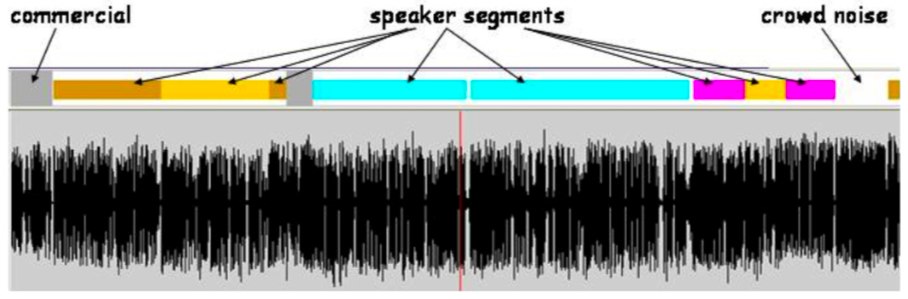
\includegraphics[width=12cm]{figures/diarization.png}
\centering
\caption{Example of audio diarization on broadcast news \cite{1677976}}
\label{fig:diarization}
\end{figure}

\section{Diarization System Modules}

Given below in figure \ref{fig:modules} is the general organization of the modules of a diarization system. Later, a brief overview of each diarization system module is given.

\begin{figure}[ht]
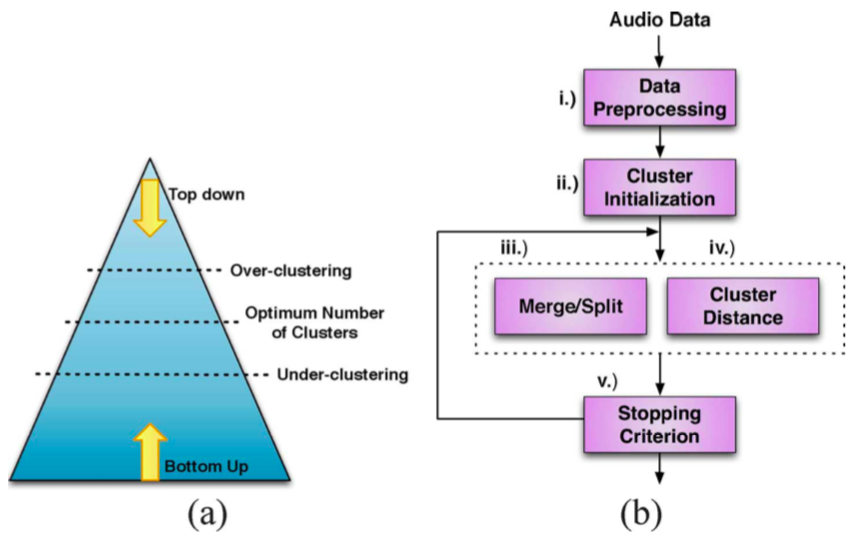
\includegraphics[width=15cm]{figures/modules.png}
\centering
\caption{General Diarization system. (a) Alternative clustering schemas. (b) General speaker diarization architecture. \cite{anguera2012speaker} }
\label{fig:modules}
\end{figure}

	\subsection{Preprocessing}
		\subsubsection{Speech Enhancement / Noise Reduction}
		A diarization system needs to address the problem of environmental noise in audio recordings. It is important to remove as much background noise as possible, but also speaker-specific information should not be lost. Also, the artefacts in denoised speech tend to reduce diarization performance. In recent years deep learning methods have partially solved the problem of artefacts, as shown in \cite{6739096}, \cite{6639038}, \cite{6665000}. But generalization ability in mismatched conditions (in terms of speaking style, interferences, interaction) is still a problem. After this stage, the enhanced speech results in increased performance for the subsequent diarization stages. 
		
		\subsubsection{Multiple Microphones}
		In the meeting domain, multiple microphones are often used from different locations of the room, so there are multiple channels of audio available to work with. Multiple microphones allow the possibility of choosing the channel with the best signal-to-noise ratio (SNR) but that also means dealing with inter-microphone delays. Many approaches have been designed to do diarization with multiple microphones. One approach performs diarization on each channel separately and merge the outputs using some algorithm. Another approach does speaker segmentation on all channels separately but only applies diarization on segments with best SNR. Some systems also combine channels to obtain a single mono channel, possibly weighing them by their SNR, then performing the diarization on it.
		
		\subsubsection{Acoustic Beamforming}
		Multiple channels usually come with inter-channel delay (which can be in the order of seconds) with arises due to the time-delay-of-arrival (TDOA) of each microphone. This is a huge problem and severely affects diarization performance. This is commonly solved by acoustic beamforming which is discussed in \cite{anguera2007acoustic}. Many people use the free tool BeamformIt \cite{anguera2006beamformit} which uses an enhanced delay-and-sum algorithm to correct misalignments.

	\subsection{Speech Activity Detection}
	Speech activity detection splits a recording into speech and nonspeech segments. This is important because this obviously has a large effect on the diarization output. The task is far from trivial since nonspeech can consist of a variety of sounds; for example in a meeting setting, it can consist of paper shuffling, door knocks, breathing, coughing, laughing etc.
	The general approach to doing speech activity detection is model-based. The binary classification models are pre-trained with external speech and non-speech data. This also makes it possible to adapt them to specific domains. This process does have a drawback because relying on external data makes the models less robust to changes in acoustic conditions. Hybrid approaches are one proposed solution, in which an energy detector is first used to label a limited amount of data for which there is high confidence in the classification. In the next step, this labelled data is used to train models that are specific to the recording event. These models are later used to obtain the final segmentation.
	
	\subsection{Segmentation}
	Another fundamental part of speaker diarization systems is speaker segmentation. The goal of this stage is to split the audio stream into speaker homogeneous segments, or in other words, detecting speaker turns. The classical approach to segmentation uses a sliding window across the speech segments, comparing consecutive windows. The comparison decides whether the two segments are better accounted by two separate models (different speakers) or a single model (same speaker) using a empirically determined threshold. Many distance metrics exist for making this decision, some of which include the $\Delta$ Bayesian Information Criterion ($\Delta$BIC) metric \cite{Chen1998SpeakerE}, generalized likelihood ratio (GLR), Kullback-Leibler (KL) divergence etc, information change rate (ICR) etc.
		
	\subsection{Clustering}

\begin{figure}[h]
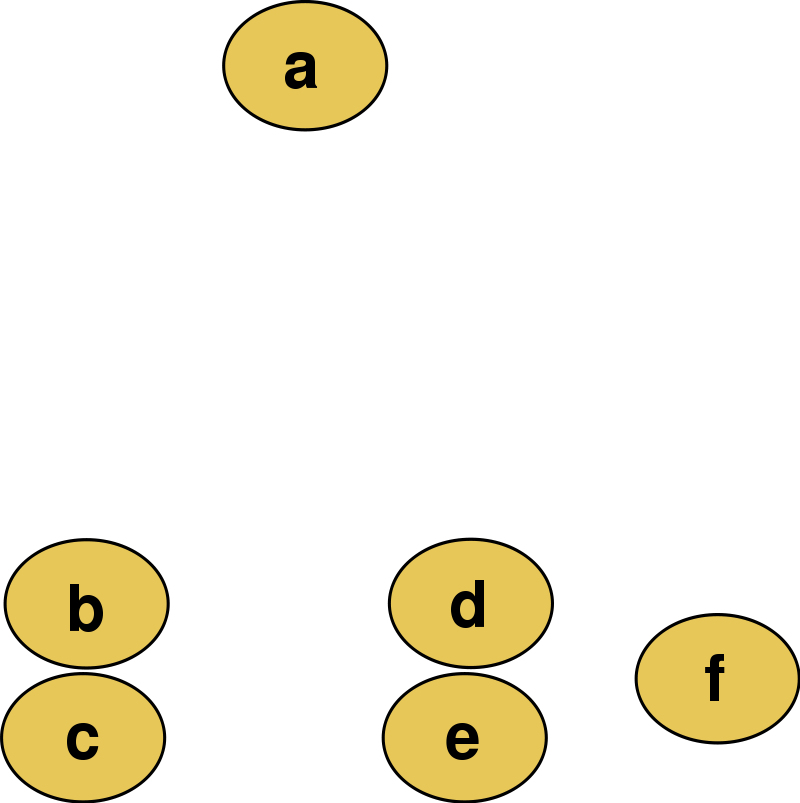
\includegraphics[width=4cm]{figures/hac-1.png}
\centering
\caption{Unclustered data \cite{wiki:hac}}
\label{fig:hac1}
\end{figure}	
	
	The segmentation step works on adjacent windows, but clustering works on the whole audio stream and works to group together all same-speaker segments. In the ideal case, every speaker has their own cluster. The same distance metrics as previous can be used here too. Most diarization systems fall in two categories: bottom-up and top-down clustering approaches. Regardless of the approach used, both of them try to converge to the optimum number of speakers, which is the actual number in the audio recording. If the final number is high than the actual number, the system is said to be under-clustered. If lower then it is called over-clustered. Both approaches are based on Hidden Markov Models (HMMs) where each state is a Gaussian Mixture Model (GMM) and represents a speaker. State transitions correspond to speaker turns. Each cluster is modelled with a GMM.
	
\begin{figure}[h]
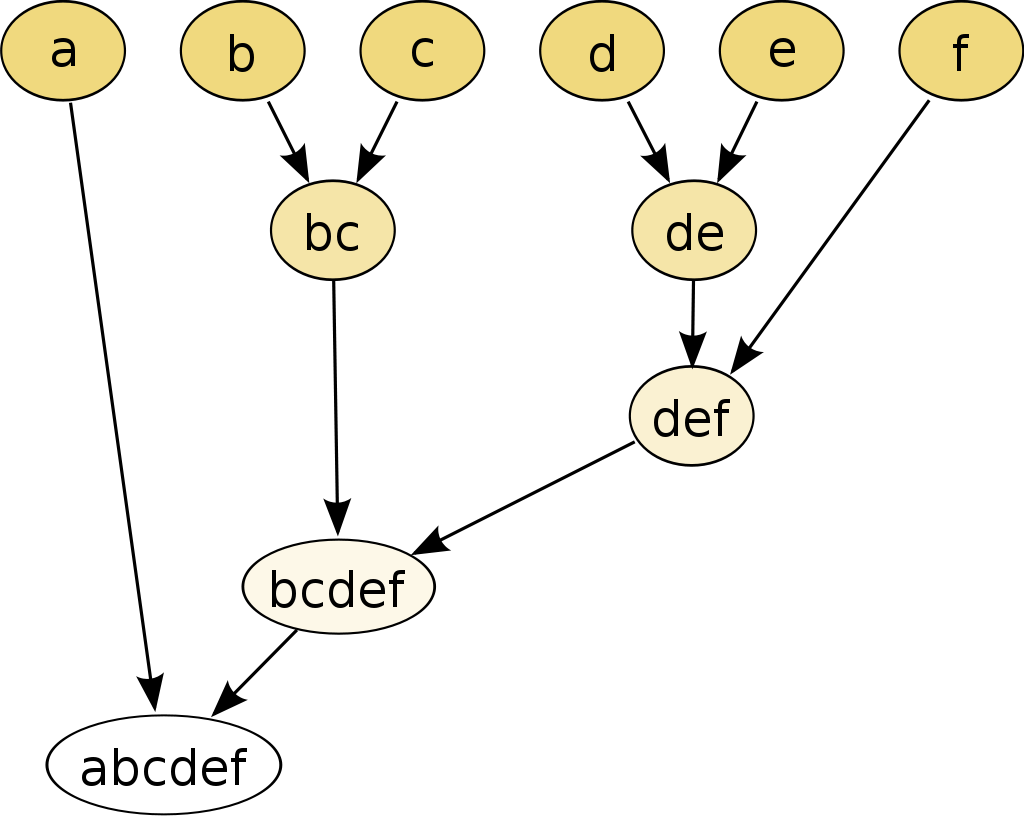
\includegraphics[width=6cm]{figures/hac-2.png}
\centering
\caption{AHC \cite{wiki:hac}}
\label{fig:hac2}
\end{figure}
	
	The bottom-up approach is the most commonly used one. It is also known as agglomerative hierarchical clustering (AHC). This approach initializes many more clusters than the actual speakers and aims at reducing the number of clusters by 1 in each iteration by merging two of the clusters. Many initializations are possible, some use k-means clustering and many use uniform initialization. Merged clusters are modelled with a GMM and use the data from the two individual clusters. Reassignment of frames to clusters is done after each cluster merge using Viterbi decoding. The whole process is repeated until some stopping criterion is reached.
		
	The top-down approach is far less popular and uses just one model (GMM) as a starting point which models the whole audio and successively adds models. Initially all segments are marked unlabelled.  Some unlabelled segments are chosen using some selection process, and used as training data for a new model (GMM). These segments are marked labelled. Viterbi alignment is interleaved and the models are re-adapted. This is continued until some stopping criterion is reached (similar to the bottom up case) or no unlabelled segments remain. Top down systems are usually out-performed by bottom up systems, but they have an advantage of being computationally efficient.
	
	Alternately, Bayesian machine learning has also been used for diarization. The key here is not making point estimates of system parameters, but instead the parameters of their distribution, also known as hyperparameters. This allows soft decisions to be taken and thus avoids a premature hard decision. However this needs computation of posterior distributions which are often too complex, and thus approximate inference methods are needed. Monte Carlo Markov Chains (MCMCs) made using Bayesian possible by computing distributions via sampling, but they are often too slow with large amount of data. An  alternative approach was Variational Bayes \cite{10.1007/11677482_27} \cite{Reynolds2009ASO} \cite{Kenny2008BayesianAO} is popular for approximating distributions, which allows approximating the intractable distribution by converting the inference problem to an optimization problem.
	
	\subsection{One-step segmentation and clustering}
	In an approach where clustering is a separate step which is performed after segmentation, there is no provision for splitting segments which contain a speaker turn, thus the quality of diarization is good only if the initial segmentation is of good quality. Since this is rarely the case, one-step segmentation and clustering approaches have been introduced which combine clustering with iterative re-segmentation. These systems perform clustering on a frame-to-cluster basis. Viterbi realignment is used to re-segment the audio based on the current clustering hypothesis, and the models are retrained based on the new segmentation. Most of the state-of-the-art diarization systems use one-step segmentation and clustering.
	
	\subsection{Speaker Representation}
		\subsubsection{GMM-UBM model}
		Early diarization systems used GMMs with cepstral features to represent speakers. However, since segments durations are small, the number of feature vectors available is often too small to estimate a GMM. To solve this, a pre-trained Universal Background Model (UBM) was introduced \cite{Reynolds:2000:SVU:2774258.2774423}, which is trained from a large number of speakers from an external dataset to capture the general variability of speech. To get the speaker model, the UBM is adapted to the speaker segments. To compute statistical similarity between GMMs, measures like KL divergence, normalized cross likelihood ratio (NCLR) can be used.
				
		\subsubsection{GMM supervectors}
		Experiments show that the means of GMMs have the most amount of speaker information by far. So the mean vectors of a GMM are concatenated into a giant vector called a GMM supervector, and it represents the GMM. Distance measures between supervectors have been investigated in \cite{5545402}. Two supervectors can only be compared if they are adapted from the same UBM.
		
		\subsubsection{i-vectors}
		The high dimensionality of supervectors is a problem for computation. \cite{5545402} uses factor analysis to reduce the dimensionality of the supervector and get a new representation into a new space called ``total variability subspace". The representation obtained is called i-vector. The parameters to do this transformation need to be learned from a training dataset. Recently i-vectors have been shown to give state-of-the-art results in speaker recognition.
				
	\subsection{Overlapping Speech}
	Most speaker diarization systems assign only one speaker to each segment. This can be considered as a fundamental limitation, since it is entirely possible for a segment to have overlapping speech from multiple speakers. In such segments, both missed speech errors and speaker identification errors occur. These segments also affect the purity of clusters of which they are a part of.
	Some strategies have been used to deal with segments of overlapping speech. In systems where ground-truth overlap detection was available, some have tried to add a second speaker to these regions by just using speaker labels of neighbouring segments. Some have also tried excluding overlapping regions from the input to the diarization system. Real overlap detection has been done in the past \cite{trueba2008handling} using a 3-state HMM-GMM system (nonspeech, non-overlapped speech, overlapped speech) with some success. Very recently, \cite{isik2016single} and \cite{hershey2016deep} talk about doing speaker separation for single-channel mixtures using a deep learning architecture called ``deep clustering".
	
	\subsection{Time-Delay Features}
	As already seen, inter-channel delays exist in multi-channel scenarios. It is possible to use these delays for speaker localization. These estimates of speaker location (assuming that speakers do not move) can be treated as alternative features.
	
	\subsection{Diarization Evaluation}
	Since 2004, the National Institute of Standards and Technology (NIST) organizes benchmark evaluations within the RT campaigns. One of the tasks is speaker diarization. Most of recent NIST RT evaluations have focussed on the conference meeting domain which is more challenging and as stated before, ``speech recognition complete". Several evaluation conditions are created using combinations of different conditions - single/multi channel audio, microphone types etc.
	
	\subsubsection{Diarization Error Rate}
		The NIST systems are evaluated using the diarization error rate (DER) metric, which is composed of three errors: missed speech (MISS), false alarm speech (FA), and speaker error (ERROR). TOTAL is the total duration of the audio recording. Missed speech is the percentage of speech that is in the ground truth but not in the prediction. False alarm speech is the percentage of speech that is in the prediction but not in the ground truth. Speaker error is the percentage of speech assigned to an incorrect speaker. Speaker error is classified into incorrectly assigned single speaker, and speaker overlap error. Speaker overlap error can be further classified as missed overlap (few speakers predicted than actual) or false alarm overlap (more speakers predicted than actual).
		From the definition of DER it is obvious that it is time-weighted. It assigns more importance to the diarization quality of speakers who have longer speaking times. Sometimes a non-scoring collar of a few milliseconds is applied on the sides of ground-truth segment boundaries to account for inconsistencies caused by imprecise start and end timestamps.
			
	$$ DER = \frac{FA + MISS + ERROR}{TOTAL} $$

	\subsubsection{Jaccard Error Rate}
	A new metric has been developed for DIHARD for use as an alternative metric called the Jaccard Error Rate (JER). This is based on the Jaccard Index \cite{hamers1989similarity}. The Jaccard Index is computed for each pair of optimal mappings between reference and system speakers. The Jaccard Error Rate is defined as 1 minus the average of these scores. It is similar to DER, but unlike DER it weighs each speaker's contribution equally regardless of how much they speak.
	
	Assume we have $N$ reference speakers, $M$ system speakers. After the optimal mappings are determined, for each reference speaker $ref$ the speaker-specific Jaccard error rate $JER_{ref}$ is computed by:
	
	$$ JER_{ref} = \frac{FA + MISS}{TOTAL} $$
	
	The Jaccard error rate is then the average of speaker specific Jaccard error rates.
	
	$$ JER = \frac{1}{N} \sum_{ref} JER_{ref} $$

\section{Summary}
	To summarize, we can see that even a seemingly simple problem statement like speaker diarization has a lot of modules doing various jobs under the hood. The core of the system is the segmentation and clustering part, which does most of the work. Diarization uses a lot of concepts from the fields of speaker identification and verification for modelling speakers.
